\documentclass[tikz,border=10pt]{standalone}
\usepackage{amsmath}
\usetikzlibrary{arrows.meta,positioning,fit,shapes,calc}

% font
%\usepackage{fourier}
\usepackage[T1]{fontenc}
\usepackage{mathpazo,mathabx}

\tikzset{
  var/.style={minimum size=8mm,inner sep=0pt,font=\small},
  arrow/.style={-Latex,thick}
}

\begin{document}
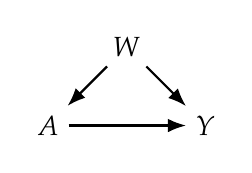
\begin{tikzpicture}
  \node[] (A)  at (0.0, 0.0) {$A$};
  \node[] (Y)  at (2, 0.0) {$Y$};
  \node[] (C)  at (1, 1) {$W$};

  \draw[arrow] (A) -- (Y);
  \draw[arrow] (C) -- (A);
  \draw[arrow] (C) -- (Y);
\end{tikzpicture}
\end{document}
